\documentclass[final]{beamer}
%% Possible paper sizes: a0, a0b, a1, a2, a3, a4.
%% Possible orientations: portrait, landscape
%% Font sizes can be changed using the scale option.
\usepackage[size=a0,orientation=portrait,scale=1.25]{beamerposter}

\usetheme{gemini}
\usecolortheme{seagull}
\useinnertheme{rectangles}

% Header colour
\definecolor{BlockHeader}{HTML}{17375E}

% Regular block: white body, dark-blue header
\setbeamercolor{block title}{fg=white,bg=BlockHeader}
\setbeamercolor{block body}{fg=black,bg=white}



% ====================
% Packages
% ====================

\usepackage[utf8]{inputenc}
\usepackage{graphicx}
\usepackage{booktabs}
\usepackage{tikz}
\usepackage{pgfplots}
\usetikzlibrary{arrows.meta,positioning,calc}

% ====================
% Lengths
% ====================

% Two unequal columns: the left column (background / related work) is
% narrower, the right column (methodology / evaluation / takeaways) is
% wider, since it carries the more important content.
% 3*\sepwidth + \colwidthleft + \colwidthright = \paperwidth
\newlength{\sepwidth}
\newlength{\colwidthleft}
\newlength{\colwidthright}
\setlength{\sepwidth}{0.015\paperwidth}
\setlength{\colwidthleft}{0.367\paperwidth}
\setlength{\colwidthright}{0.588\paperwidth}

\newcommand{\separatorcolumn}{\begin{column}{\sepwidth}\end{column}}

% ====================
% Logo (optional)
% ====================

% use this to include logos on the left and/or right side of the header:
\logoleft{
\includegraphics[height=5cm]{logos/UOfT_logo.png}}
\logoright{
\includegraphics[height=5cm]{logos/tcig_final.png}}

% ====================
% Poster background
% ====================
\usebackgroundtemplate{%
	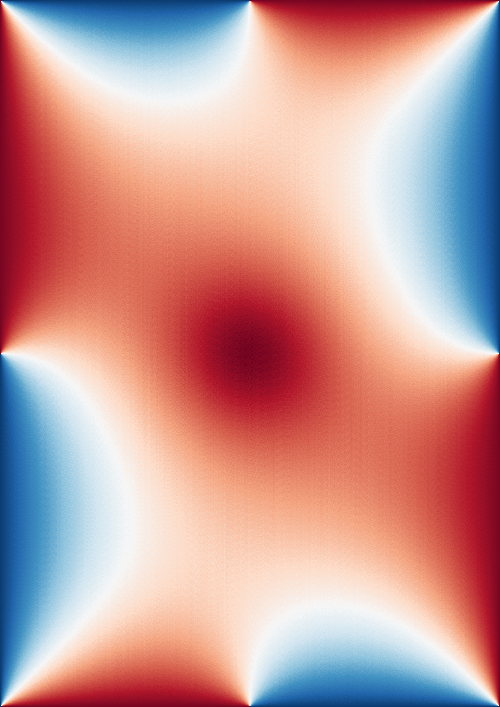
\includegraphics[width=\paperwidth,height=\paperheight]{Images/rectangle_piecewise_g_solution.png}
}

% ====================
% My own customization
% - BibLaTeX
% - Boxes with tcolorbox
% - User-defined commands
% ====================
\input{custom-defs.tex}

\setdefboxbasecolor{blue}

%% Reference Sources
\addbibresource{refs.bib}
\renewcommand*{\bibfont}{\footnotesize}
\renewcommand{\pgfuseimage}[1]{\includegraphics[scale=2.0]{#1}}

% ====================
% Design elements re-used across blocks
% ====================

% A highlighted "callout" box with a coloured left rule, used for the
% key equations / convergence conditions that should catch the eye.
\newtcolorbox{eqbox}{%
	colback=white, colframe=BlockHeader,
	boxrule=0pt, leftrule=3pt, arc=0pt, outer arc=0pt,
	boxsep=4pt, left=10pt, right=8pt, top=6pt, bottom=6pt
}

% A dashed placeholder box standing in for a not-yet-measured figure.
\newcommand{\placeholderfig}[3]{%
	\begin{tikzpicture}
		\node[draw, dashed, thick, gray, minimum width=#1, minimum height=#2,
			align=center, text width=0.9*#1, font=\itshape\small, gray] {#3};
	\end{tikzpicture}%
}

\title{A Source-Iteration Framework for Monte Carlo Helmholtz Solvers via Walk-on-Boundary}

\author{Pratham Gupta\inst{1} \and Prashanth Shyamala\inst{2} \and Benjamin Attal\inst{2} \and Jorge~Garcia-Pueyo\inst{3} \and David Lindell\inst{2}}

\institute{\textsuperscript{1}Indian Institute of Science \quad \textsuperscript{2}University of Toronto \quad \textsuperscript{3}University of Zaragoza}

\begin{document}

% Force reference numbering to match the intended [1]-[5] order.
\nocite{Sawhney2020,Sugimoto2023,Osnabrugge2016,Yang2017,Jakob2022}

\begin{frame}[t]

	\begin{columns}[t]
		\separatorcolumn

		\begin{column}{\colwidthleft}

			\begin{block}{The problem}

				We solve the inhomogeneous Helmholtz wave equation $(\Delta + k^2)u = -f$, the PDE governing time-harmonic waves --- sound, light, seismic.

				\begin{itemize}
					\item \textbf{FEM/FDM discretize the entire domain.} Holding accuracy as $k \to \infty$ needs DOFs growing faster than $k^d$ (the pollution effect) --- slow, memory-heavy, and the indefinite linear system is hostile to solve. Adjoint/FWI-style inversion must additionally store the full wavefield, $O(k^d)$ per frequency, and runs out of memory at scale.
					\item \textbf{Monte Carlo has no global dependence.} Grid-free, output-sensitive estimators --- Walk-on-Spheres/Walk-on-Boundary \parencite{Sawhney2020} --- evaluate $u$ at any query point directly, with no mesh and no global linear system to assemble or store.
					\item \textbf{But existing MC methods fail for Helmholtz.} The boundary operator $A$ is sign-indefinite, so $\rho(A) \ge 1$ and the Neumann series $\mu = \sum_{n\ge0} A^n b$ diverges --- the walk never converges.
				\end{itemize}

			\end{block}

			\begin{block}{Walk on Boundary}

				Walk-on-Boundary recasts the BVP as an integral equation along $\partial\Omega$,
				$$\mu(x) - \int_{\partial\Omega} K(x,y)\,\mu(y)\,dS_y = b(x), \quad x \in \partial\Omega$$
				$$\big(\text{compactly } (I-A)\mu = b\big),$$
				and estimates the density $\mu$ with unbiased random walks on $\partial\Omega$ that realize the Neumann series $\mu = \sum_{n \ge 0} A^n b$, without ever discretizing the interior of $\Omega$.

				\begin{figure}
					\centering
					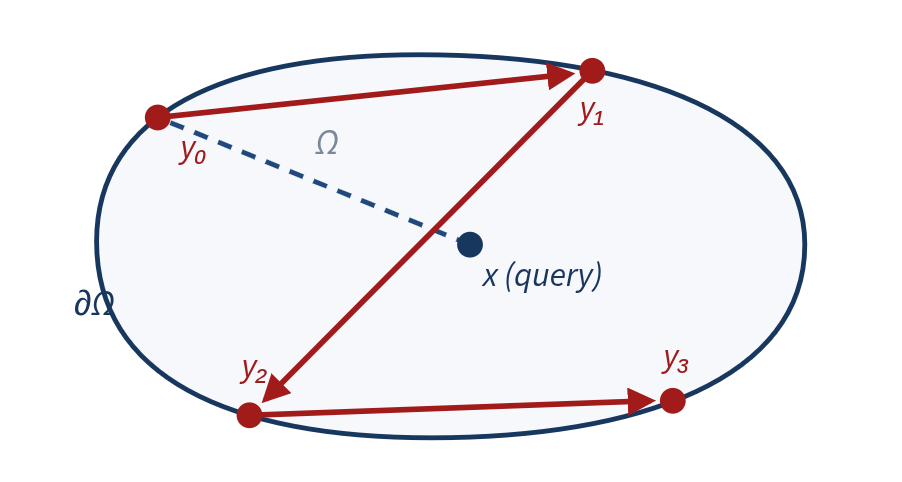
\includegraphics[width=0.55\linewidth]{Images/Helmholtz WoB Poster-selection.png}
				\end{figure}

				\heading{Why it breaks for Helmholtz}

				\begin{eqbox}
					\[
						(I - A)\mu = b, \qquad \mu = \sum_{n \ge 0} A^n b \qquad \text{converges only if } \rho(A) < 1
					\]
				\end{eqbox}

				\begin{itemize}
					\item At moderate to high $k$ the indefinite kernel gives $\rho(A) \ge 1$: the series \textbf{diverges}, and deep walks estimating $A^n$ have unbounded variance --- the failure the Convergent Born Series \parencite{Osnabrugge2016} first exposed.
				\end{itemize}

			\end{block}

			\begin{block}{Related Work}

				\begin{itemize}
					\item \textbf{Grid-free MC solvers.} WoS for (screened) Poisson \parencite{Sawhney2020}; Walk-on-Stars adds Neumann and Robin data.
					\item \textbf{Walk-on-Boundary.} Practical boundary-integral estimator for Dirichlet / Neumann / Robin data \parencite{Sugimoto2023}; convergence guarantees are missing for indefinite operators.
					\item \textbf{Convergent Born Series.} Complex wavenumber $k_0^2 + i\varepsilon$ and $\gamma = (i/\varepsilon)V$ force $\rho(M) < 1$ unconditionally \parencite{Osnabrugge2016} --- the deterministic precedent for my shift.
					\item \textbf{Closest precedent.} WoS for Helmholtz / Yukawa via the Duffin correspondence \parencite{Yang2017} --- but tied to constant potentials.
				\end{itemize}

			\end{block}

			\begin{block}{References}
				\setlength{\bibitemsep}{0pt}
				\setlength{\bibparsep}{0pt}
				\printbibliography[heading=none]
			\end{block}

		\end{column}

		\separatorcolumn

		\begin{column}{\colwidthright}

			\begin{block}{Methodology}

				\textbf{The source iteration, one turn of the loop} \hfill {\small\itshape one iteration = one operator apply}

				\vspace{1ex}
				\begin{figure}
					\centering
					\begin{tikzpicture}[
						remember picture,
						node distance=12mm and 12mm,
						box/.style={draw, rounded corners, align=center, minimum height=2.3cm,
							minimum width=5cm, text width=9cm, fill=white},
						hl/.style={box, draw=BlockHeader, line width=1.2pt, fill=BlockHeader!8},
						>=Latex
					]
						\node[box] (mu) {current density $\mu^n$};
						\node[hl, right=of mu] (wob) {\textbf{one forward WoB step}\\[3pt] sample $y \sim p$,\\ estimate $A\mu^n$};
						\node[box, right=of wob] (res) {residual\\[2pt] $r^n = (I-A)\mu^n - b$};
						\node[box, right=of res] (shift) {complex shift\\[2pt] $\mu^{n+1} = \mu^n - \omega r^n$};

						\draw[->] (mu) -- (wob);
						\draw[->] (wob) -- (res);
						\draw[->] (res) -- (shift);

						% \draw[->] (shift.south) .. controls +(0,-3.8) and +(0,-3.8) .. (mu.south);
                        \draw[->] (shift.south) -- ++(0,-20mm) -| (mu.south);

						\node[font=\footnotesize\itshape, align=center]
							at ($(mu.south)!0.5!(shift.south) + (0,-3.2)$)
							{repeat: variance capped, no deep walks};

						\node[font=\footnotesize\itshape, align=center, text width=5.2cm]
							at ($(res.north)!0.5!(shift.north) + (0,2.9)$)
							{stop when $\|r^n\|$ is small $\to$ evaluate $u(x)$};
					\end{tikzpicture}
				\end{figure}

				\definecolor{PosterNavy}{HTML}{17375E}
				\definecolor{PosterBlue}{HTML}{1F497D}
				\definecolor{PosterRed}{HTML}{A11B1B}
				\begin{columns}[t]
					\begin{column}{0.32\colwidthright}
						\centering
						\tikz[remember picture]\node[font=\small\itshape] (cachedas) {cached as:};\par\vspace{4pt}
						\begin{tikzpicture}[scale=2.05, baseline=(current bounding box.north)]
							\node[font=\bfseries\small, PosterRed] at (2,0.5) {array $\mu$, $O(M)$};
							\foreach \i in {0,...,8} {
								\pgfmathsetmacro{\fillc}{\i==2 ? "PosterRed!55!white" : "PosterBlue!8!white"}
					A			\draw[PosterBlue, thin, fill=\fillc] (\i*0.45,-0.75) rectangle ++(0.4,0.75);
							}
						\end{tikzpicture}\par\vspace{10pt}
						\begin{tikzpicture}[scale=1.42, baseline=(current bounding box.north)]
							\node[font=\bfseries\small, PosterRed] at (3,3.5) {hash-grid MLP, $O(1)$};
							\draw[gray!60] (0,0) grid (3,3);
							\fill[PosterRed] (1.5,1.5) circle (2pt);
							\foreach \y in {0.5,1.5,2.5} \fill[PosterBlue!15!white,draw=PosterBlue] (3.9,\y) circle (8pt);
							\foreach \y in {0.9,2.1} \fill[PosterBlue!15!white,draw=PosterBlue] (4.9,\y) circle (8pt);
							\fill[PosterBlue!15!white,draw=PosterBlue] (5.9,1.5) circle (8pt);
							\foreach \y in {0.5,1.5,2.5} \foreach \yy in {0.9,2.1}
								\draw[gray!50,thin] (3.9,\y) -- (4.9,\yy);
							\foreach \yy in {0.9,2.1}
								\draw[gray!50,thin] (4.9,\yy) -- (5.9,1.5);
							\foreach \y in {0.5,1.5,2.5}
								\draw[gray!50,thin] (1.5,1.5) -- (3.9,\y);
						\end{tikzpicture}
					\end{column}
					\begin{column}{0.32\colwidthright}
						\centering
						\begin{tikzpicture}[scale=2.5, baseline=(current bounding box.north)]
							\draw[gray!40,-{Latex[length=2mm]}] (-1.6,0) -- (1.6,0) node[right,font=\small] {Re};
							\draw[gray!40,-{Latex[length=2mm]}] (0,-1.6) -- (0,1.6) node[above,font=\small] {Im};
							\draw[dashed, PosterNavy, thick] (0,0) circle (1);
							\foreach \p in {(1.25,0.55),(-0.4,1.35),(1.4,-0.35),(-1.3,-0.6),(0.3,1.5)}
								\fill[PosterRed] \p circle (2.5pt);
							\node[below,font=\small] at (0,-1.7) {$\rho(A) \ge 1$: diverges};
						\end{tikzpicture}
					\end{column}
					\begin{column}{0.32\colwidthright}
						\centering
						\begin{tikzpicture}[scale=2.5, baseline=(current bounding box.north)]
							\draw[gray!40,-{Latex[length=2mm]}] (-1.6,0) -- (1.6,0) node[right,font=\small] {Re};
							\draw[gray!40,-{Latex[length=2mm]}] (0,-1.6) -- (0,1.6) node[above,font=\small] {Im};
							\draw[dashed, PosterNavy, thick] (0,0) circle (1);
							\foreach \p in {(0.55,0.3),(-0.4,0.35),(0.45,-0.4),(-0.3,-0.35)}
								\fill[PosterBlue] \p circle (2.5pt);
							\node[below,font=\small] at (0,-1.7) {after $\omega$-shift: $\rho(M) < 1$};
						\end{tikzpicture}
					\end{column}
				\end{columns}

				\begin{tikzpicture}[remember picture, overlay]
					\draw[->, PosterRed, thick] (mu.south) to[out=-90, in=90] (cachedas.north);
				\end{tikzpicture}

				\vspace{0.5ex}
				\begin{eqbox}
					\begin{align*}
						\mu^{n+1} &= \mu^n - \omega\left[(I-A)\mu^n - b\right] \\
						M &= I - \omega(I-A), \qquad \rho(M) < 1 \\
						\widehat{A\mu^n} &= \frac{K(x,y)\,\mu^n(y)}{p(y)}, \qquad y \sim p
					\end{align*}
				\end{eqbox}

				{\small\itshape A complex $\omega$ rotates and rescales the spectrum of $I-A$ into the unit disk about $1$ --- the stochastic analog of the CBS $\varepsilon$-shift \parencite{Osnabrugge2016}.}

				\vspace{1ex}
				{\small\itshape One boundary sample per apply: unbiased, matrix-free, variance independent of $n$.}

				\begin{itemize}
					\item \textbf{No deep walks.} Every operator apply is one forward WoB step, so per-iteration variance is capped --- the exponential blow-up of estimating $A^n$ disappears.
					\item \textbf{Warm starts.} Bootstrap $\mu^0$ from a geometrical-optics / Kirchhoff approximation, a neighbouring frequency, or a learned cache $\hat\mu_\theta$ trained by a semi-gradient residual loss.
					\item \textbf{Implementation.} Matrix-free applies and forward walks on Dr.Jit \parencite{Jakob2022} with Mitsuba-style ray tracing: JIT-compiled, GPU/CPU-retargetable, differentiable.
				\end{itemize}

			\end{block}

			\begin{block}{Evaluation}

				{\small\itshape What I will trust as evidence --- figures and table are placeholders, not measurements.}

				\vspace{1ex}
				\begin{columns}[t]
					\begin{column}{0.48\colwidthright}
						\begin{figure}
							\centering
							\placeholderfig{6cm}{4cm}{Figure 1 --- residual vs.\ iteration (placeholder)}
							\caption{$\log\|(I-A)\mu^n - b\|$ vs.\ iteration $n$, source iteration against the Neumann series over $\rho(A) \in \{0.5,\dots,1.5\}$. Falsifiable prediction: Neumann curves turn upward at $\rho \ge 1$; source iteration descends at every $\rho$.}
						\end{figure}
					\end{column}
					\begin{column}{0.48\colwidthright}
						\begin{figure}
							\centering
							\placeholderfig{6cm}{4cm}{Figure 2 --- $\rho(M)$ over the complex $\omega$ plane (placeholder)}
							\caption{Measured decay rate $\rho(M)$ as a function of $\{\mathrm{Re}\,\omega, \mathrm{Im}\,\omega\}$. Prediction: a convergent basin bounded by the contour $\rho(M)=1$, with an optimum $\omega^\star$ inside it.}
						\end{figure}
					\end{column}
				\end{columns}

				\begin{table}
					\centering
					\begin{tabular}{lcccc}
						\toprule
						\textbf{Method} & $\rho = 0.7$ & $\rho = 0.95$ & $\rho = 1.05$ & $\rho = 1.3$ \\
						\midrule
						Neumann-series WoB & converges (slow) & converges (very slow) & \textcolor{red}{diverges} & \textcolor{red}{diverges} \\
						Source iteration (tuned $\omega$) & converges & converges & converges & converges \\
						\bottomrule
					\end{tabular}
					\caption{(Illustrative placeholder.) Outcome vs.\ spectral-radius sweep --- the crossover at $\rho = 1$ is the test.}
				\end{table}

				\begin{itemize}
					\item \textbf{Reference solutions.} Analytic fields where they exist, otherwise a dense deterministic boundary-element solve --- error reported against both, never against a single baseline.
					\item \textbf{Controls.} Sweep $\rho(A)$ across the $\rho = 1$ boundary; report per-iteration variance and sample counts, so convergence claims cannot hide behind extra samples.
				\end{itemize}

			\end{block}

			\begin{block}{What it means}

				\begin{enumerate}
					\item \textbf{Convergence becomes a design choice, not a property of the domain.} One complex scalar $\omega$ buys $\rho(M) < 1$ where the Neumann series has none.
					\item \textbf{Robustness is paid for in rate.} Following the CBS law $\Delta r = 2k_0/\varepsilon$, a larger shift guarantees convergence but slows each iteration --- warm starts buy the rate back near $\rho \approx 1$.
					\item \textbf{Open questions I want to discuss.} How far does a scalar $\omega$ stretch before an operator-valued shift is needed for heterogeneous media (Lippmann--Schwinger), and can $\hat\mu_\theta$ warm-start inverse problems without biasing gradients?
				\end{enumerate}

			\end{block}

		\end{column}

		\separatorcolumn
	\end{columns}
\end{frame}
\end{document}
